\chapter{Fundamentos}

Neste capítulo são estabelecidos os principais conceitos utilizados ao longo do trabalho. Será conduzido uma breve abordagem sobre os fundamentos de serialização de dados; seguido pelo formato de representação JSON; o estilo de arquitetura baseado em recursos e formas para descrição de seus metadados.

\section[Serialização de Dados]{Serialização de Dados}

Na ciência da computação, serialização de dados é um processo de tradução usado para converter estruturas de dados\footnote{
  Uma estrutura de dados é uma forma abstrata de representar e organizar dados. Seu objetivo é ajudar a reduzir complexidade, podendo armazenar dados de diferentes tipos, como números, strings ou até mesmo outras estruturas de dados.
} em formatos que possam ser armazenados, transmitidos e reconstruídos por um mesmo ou por outro ambiente computacional. \cite{Cline2016}

Dados serializados normalmente têm um tempo de vida maior que suas aplicações de origem e, ao serem armazenados em disco ou transmitidos pela rede, possuem representação diferente do que sua estrutura em memória. Para se ler dados serializados em memória é preciso realizar o processo inverso, também chamado de desserialização, onde estes passam a ser representados por estruturas da linguagem de execução. \cite{Guller2016}
  
\begin{figure}[H]
  \centering
  \smartdiagramset{circular distance=2cm,uniform arrow color=true,arrow line width=1pt,arrow color=gray!50!black,uniform color list=white for 6 items,font=\small,text width=2.0cm,module minimum width=2.0cm,module minimum height=1.5cm,arrow tip=to}
  \smartdiagram[flow diagram:horizontal]{Estrutura de dados,Serialização,Estrutura serializada,Desserialização}
  \caption{Processo de serialização e desserialização}
\end{figure}

Este processo, embora demande tempo, permitiu que aplicações fizessem o consumo de informações de forma distribuída, contribuindo com o aumento do volume de dados que circulam pela internet. Além disso, fez-se necessária a seleção adequada de formatos de serialização cuja estrutura não prejudicasse o desempenho de aplicações na busca por dados. \cite{SumarayMakki2012}

Segundo a Cisco Systems, de 2014 para 2015, houve um aumento de 21\% no volume de tráfego de dados registrados apenas por seus aparelhos. As categoria Web, Email e Data foram responsáveis por representar aproximadamente 7,558 petabytes de dados transmitidos por seus clientes durante um mês. \cite{Cisco2016}

Para suprir esta alta demanda, diversos formatos de serialização foram introduzidos para melhor atender os problemas de desempenho experienciados por serviços. Dentre eles, tempo de serialização e desserialização, tamanho de transferência, flexibilidade de uso, facilidade de leitura, automação, suporte para linguagem, entre outros. \cite{Guller2016}

\begin{table}[ht!]
  \centering
  \resizebox{\columnwidth}{!}{
    \begin{tabular}{|c|c|c|c|c|}
      \hline
      Formato & Especificação & Codificação & Legibilidade & Esquema/IDL \\
      \hline
      XML & Padronizada & Textual & Sim & Sim \\
      \hline
      JSON & Padronizada & Textual & Sim & Parcial \\
      \hline
      YAML & Padronizada & Textual & Sim & Parcial \\
      \hline
      Avro & Padronizada & Binário & Não & Sim \\
      \hline
      P. Buffers & Padronizada & Binário & Parcial & Sim \\
      \hline
      Thrift & Não Padronizada & Binário & Parcial & Sim \\
      \hline
    \end{tabular}
  }
  \caption{Comparação de formatos de serialização}
\end{table}

Para melhor entender cada formato, será feita uma abordagem sobre algumas das categorias de classificação utilizadas para estudar o desempenho dos formatos existentes hoje em dia. \\

\textbf{Especificação} \\

Um formato pode ter sua especificação classificada como padronizada ou não padronizada. Uma especificação padronizada é regida por requisitos que auxiliam na reprodutibilidade do processo em outras linguagens para maximização da compatibilidade e minimização de erros. Ao contrário, dada uma linguagem de programação, não é garantido que sua implementação esteja seguindo os padrões e poderá ser considerado como não padronizada. \cite{McDermid1991} \\

\textbf{Codificação} \\

Codificação é o processo de sequenciamento de caracteres usado na representação dos dados transmitidos ou armazenados. É possível classificar em dois tipos: textuais e binários. Formatos baseados em texto podem ser lidos diretamente através de editores de texto. Já um formato binário faz o uso intensivo da codificação e decodificação para salvar espaço. \cite{Queiros2014} \\

\textbf{Legibilidade} \\

Ao representar estruturas de dados em formatos de serialização para que máquinas possam fazer a leitura, não é garantido, no entanto, que esta representação também seja legível por seres humanos.

Para que um formato seja legível por humanos (\textit{human-readable}), além de máquinas, pessoas devem conseguir ler e dizer o que está sendo representado na estrutura, mesmo fora de contexto. Para desenvolvedores, este detalhe é essencial no processo de debugging\footnote{
  Depuração é o processo de encontrar e reduzir defeitos num aplicativo de software ou mesmo em hardware.
}. Nota-se que a leitura de um formato é diferente de seu entendimento, uma vez que nem todos os formatos possuem maneiras de descrever seus metadados. O formato JSON, por exemplo, é baseado em texto e tem como objetivo a facilidade de uso e legibilidade por desenvolvedores. Nem sempre, contudo, é possível identificar o que está sendo representado em suas estruturas. \cite{SumarayMakki2012} \\

\textbf{Esquema/IDL} \\

Com objetivo de entender o que está sendo representado, alguns formatos disponibilizam na sua especificação maneiras de descrever metadados. Esta categoria é importante principalmente para que máquinas consigam inferir quais estruturas estão sendo lidas e, assim, tomar decisões de forma autônoma.

Um formato descritivo normalmente disponibiliza estruturas como esquemas IDL\footnote{
  Linguagem de descrição utilizada para descrever a interface dos componentes de um software.
} para descrição da própria representação. À medida que estas descrições são incorporadas dentro da mesma representação, é possível classificar estes formatos como sendo auto-descritivos. \cite{Rentachintala2014}

\section{JSON}

JSON ou Javascript Object Notation é um formato de serialização de dados human-readable baseado em texto com especificação padronizada e parcialmente descritivo. Foi desenvolvido por Douglas Crockford com o objetivo de representar dados em uma maneira simples, leve e flexível através da redução na sobrecarga de marcações comparado ao formato XML.

Por ter se adaptado bem no ambiente de aplicações distribuídas, este formato acabou sendo amplamente utilizado em serviços como principal forma de representação de dados serializados. \cite{Duvander2013}

Na sua essência, o JSON foi construído com base em quatro tipos primitivos de dados e outros dois para composição. Cada tipo possui seu respectivo correspondente na maioria das linguagens de programação, embora possam ser identificados por nomes diferentes. \cite{Droettboom2015}

\begin{table}[H]
  \centering
  \begin{tabular}{|c|c|c|c|c|}
    \hline
    Tipo & Exemplo de Valor \\
    \hline
    object & \mintinline[fontsize=\footnotesize]{text}{ {"chave1": "valor1", "chave2": "valor2"} } \\
    \hline
    array & \mintinline[fontsize=\footnotesize]{text}{ ["primeiro", "segundo", "terceiro"] } \\
    \hline
    number & \mintinline[fontsize=\footnotesize]{text}{ 1, -1, 2.9999 } \\
    \hline
    string & \mintinline[fontsize=\footnotesize]{text}{ "Isso é uma string" } \\
    \hline
    boolean & \mintinline[fontsize=\footnotesize]{text}{ true, false } \\
    \hline
    null & \mintinline[fontsize=\footnotesize]{text}{ null } \\
    \hline
  \end{tabular}
  \caption{Tipos de valores em JSON}
\end{table}

Através da composição de listas, objetos e tipos primitivos, consegue-se representar complexas estruturas de dados. Não existe, no entanto, um único padrão de representação. Dada uma estrutura, é possível representá-la de inúmeras maneiras. A seguir estão duas formas diferentes de representação em JSON de uma entidade “pessoa”:
 \cite{Droettboom2015}

\begin{figure}[H]
  \centering
  \begin{minted}[frame=single,framesep=10pt,fontsize=\footnotesize]{text}
    {
      "nome": "Mateus Maso",
      "aniversario": "25 de março de 1992",
      "cidade": "Florianópolis, SC, Brasil"
    }
  \end{minted}
  \caption{Primeiro exemplo de representação JSON}
\end{figure}

\begin{figure}[H]
  \centering
  \begin{minted}[frame=single,framesep=10pt,fontsize=\footnotesize]{text}
    {
      "nome": "Mateus",
      "sobrenome": "Maso",
      "nascimento": "25-03-1992",
      "cidade": {
        "nome": "Florianópolis",
        "estado": "SC",
        "pais": "Brasil"
      }
    }
  \end{minted}
  \caption{Segundo exemplo de representação JSON}
\end{figure}

Ambas representações são válidas, apesar da figura 4 estar representando os dados em uma estrutura um pouco mais formal. No entanto, por ser um formato não descritivo, a responsabilidade de entender o que está sendo representado vai depender da análise crítica ou conhecimento prévio dos desenvolvedores. Já uma máquina, sem conhecer o contexto, não saberia como interpretar os dados de forma correta. \cite{Droettboom2015}

Para resolver isso, será abordado em seguida um dos formatos existentes hoje em dia para a descrição de estruturas JSON.

\section[JSON Schema]{JSON Schema}

JSON Schema é uma linguagem de definição projetada para descrever estruturas de dados JSON por meio de esquemas. Proposta em 2009 por Kris Zyp, teve como objetivo fornecer um contrato para que aplicações soubessem como trabalhar e interagir com estruturas de dados. Por meio deste, é possível prever representações e assim realizar operações de validação, documentação, navegação por \textit{hyperlinks} e controle de iteração. \cite{Zyp2013}

Por ser uma linguagem de simples uso, para modelar um esquema basta construir um objeto JSON utilizando um subconjunto válido de chaves especias descritas pela linguagem. No entanto, funcionalidades como descrição de estruturas multimídia\footnote{
 Capaz de reunir diversas mídias, como imagens, textos, vídeos e audio digital, por exemplo.
} e a navegação de dados são apenas disponibilizadas no formato JSON Hyper-Schema, uma variação da linguagem de especificação. \cite{Jackson2016}

\begin{figure}[H]
  \centering
  \begin{minted}[frame=single,framesep=10pt,fontsize=\footnotesize]{text}
    {
      "\$schema": "http://json-schema.org/draft-04/schema#",
      "title": "Pessoa",
      "description": "Uma pessoa",
      "type": "object",
      "required": ["nome", "aniversario"],
      "properties": {
        "nome": {
          "type": "string"
        },
        "aniversario": {
          "type": "string"
        },
        "cidade": {
          "type": "string"
        }
      }
    }
  \end{minted}
  \caption{JSON Schema para Figura 3}
\end{figure}

\begin{figure}[H]
  \centering
  \begin{minted}[frame=single,framesep=10pt,fontsize=\footnotesize]{text}
    {
      "\$schema": "http://json-schema.org/draft-04/hyper-schema#",
      ...,
      "properties": {
        ...,
        "foto": {
          "media": {
            "binaryEncoding": "base64",
            "type": "image/png"
          }
        }
      },
      "links": [
        {
          "rel": "foto",
          "href": "/{id}.png",
          "mediaType": "image/png"
        }
      ]
    }
  \end{minted}
  \caption{JSON Hyper-Schema para Figura 3}
\end{figure}

Ao exemplo das figuras 4 e 5, ambos os esquemas asseguram que, dada uma estrutura JSON, para que esta seja reconhecida como uma entidade “pessoa”, deve conter as propriedades "nome" e "aniversario" com valores do tipo "string". Já na figura 5, além das estruturas definidas pela figura 4, é descrita uma nova propriedade "foto" do tipo multimídia, além de como navegar em busca desta informação.

Em casos onde a complexidade de um esquema começa a crescer, é comum a definição de sub-esquemas através da chave “definitions”. Desta forma, podem ser referenciadas pela chave "\$ref" permitindo o reuso de estruturas dentro de um esquema. Vale lembrar que a chave “definitions” é apenas um mecanismo útil para definir esquemas em um lugar comum, entretanto, não sugerem que estas propriedades sejam validadas em um objeto ao menos que referenciadas em outras estruturas do esquema. \cite{Leach2014}

\begin{figure}[H]
  \centering
  \begin{minted}[frame=single,framesep=10pt,fontsize=\footnotesize]{text}
    {
      "\$schema": "http://json-schema.org/draft-04/hyper-schema#",
      ...,
      "definitions": {
        "cidade": {
          "type": "string",
          "properties": {
            "nome": { "type": "string" },
            "estado": { "type": "string" },
            "pais": { "type": "string" }
          }
        }
      },
      "properties": {
        ...,
        "cidade": {
          "\$ref": "#/definitions/cidade"
        }
      },
      "links": [
        ...,
        {
          "rel": "cidade",
          "href": "/{id}/cidade",
          "targetSchema": {
            "\$ref": "#/definitions/cidade"
          }
        }
      ]
    }
  \end{minted}
  \caption{JSON Hyper-Schema para Figura 4 usando \$ref}
\end{figure}

Como boa prática, é recomendado (mas não necessário) o uso da chave especial “\$schema” para determinar quando uma estrutura JSON está sendo representada em forma de esquema. Na tabela 3 são descritas algumas das chaves especiais usadas para descrever objetos em esquemas. \cite{Droettboom2015}

\begin{table}[ht!]
  \centering
  \begin{tabular}{|c|c|}
    \hline
    Chave & Descrição \\
    \hline
    \$schema & Identificador de versão \\
    \hline
    type & Tipo de dado \\
    \hline
    title & Nome da estrutura \\
    \hline
    description & Propósito da estrutura \\
    \hline
    required & Lista de propriedades com presença obrigatória \\
    \hline
    properties & Propriedades usadas para validar uma estrutura \\
    \hline
    definitions & Propriedades (sub-esquemas) para referência \\
    \hline
    ... & ... \\
    \hline
    links & Lista de Link Description Objects (LDO) \\
    \hline
  \end{tabular}
  \caption{Subconjunto de chaves especiais JSON Schema}
\end{table}

De certa forma, JSON Schema continua sendo uma das únicas tentativas sérias de propor uma linguagem de definição para o formato JSON. Contudo, ainda está longe de ser considerada padrão, mas já há um número crescente de aplicações que suportam o formato, além de uma quantidade significativa de ferramentas que permitem sua validação. \cite{PezoaEtAl2016}

Vale lembrar também que, segundo Leach, com o recente surgimento de grandes formatos de descrição de APIs ao longo dos últimos anos, JSON Hyper-Schema tem-se tornado uma ótima opção para descrever a navegação para acesso de interfaces, como por exemplo nome de método, estruturas de chamada e resposta, entre outros relacionamentos. \cite{Leach2014}

Nas próximas seções será abordado um dos estilos de arquitetura mais utilizados hoje em dia em APIs Web, além de soluções encontradas no mercado para descrição deste tipo de API em serviços.

\section{REST}

REST (\textit{Representational State Transfer}) é um estilo de arquitetura usada para a comunicação de sistemas distribuídos através do protocolo HTTP. Foi introduzido por Roy Fielding em 2000 com o objetivo de oferecer às aplicações web um modelo de interface de acesso baseada em recursos. Além disso, descreve seis tipos de restrições que serviços deveriam aplicar para ganho de performance, escalabilidade, simplicidade, modificabilidade, visibilidade, portabilidade e confiabilidade.

Em virtude de causar grande repercussão após sua publicação, o termo REST, segundo Richardson, acabou sofrendo diversas interpretações durante o tempo e sua descrição foi representada de formas não originalmente propostas por Fielding \cite{RichardsonEtAl2013}. Alguns descrevem que serviços que violam essas restrições não podem ser considerados RESTful. Para Wildermuth, apesar de reconhecer as vantagens de cada restrição, serviços web devem usá-los de forma pragmática \cite{Wildermuth2015}.

Ao ser introduzido no mercado de APIs, REST acabou se adaptando bem por ter se mostrado uma solução de fácil acesso em clientes web, dispositivos móveis e de IoT\footnote{
  Do inglês \textit{Internet of Things} (Intenet das Coisas).
}. Segundo Pautasso, a eliminação da complexidade existente em Web Services antes de sua publicação em 2000 fez com que REST fosse considerado um dos principais responsáveis pela popularização de arquiteturas orientada a serviços. \cite{PautassoEtAl2008}

\begin{figure}[H]
  \centering    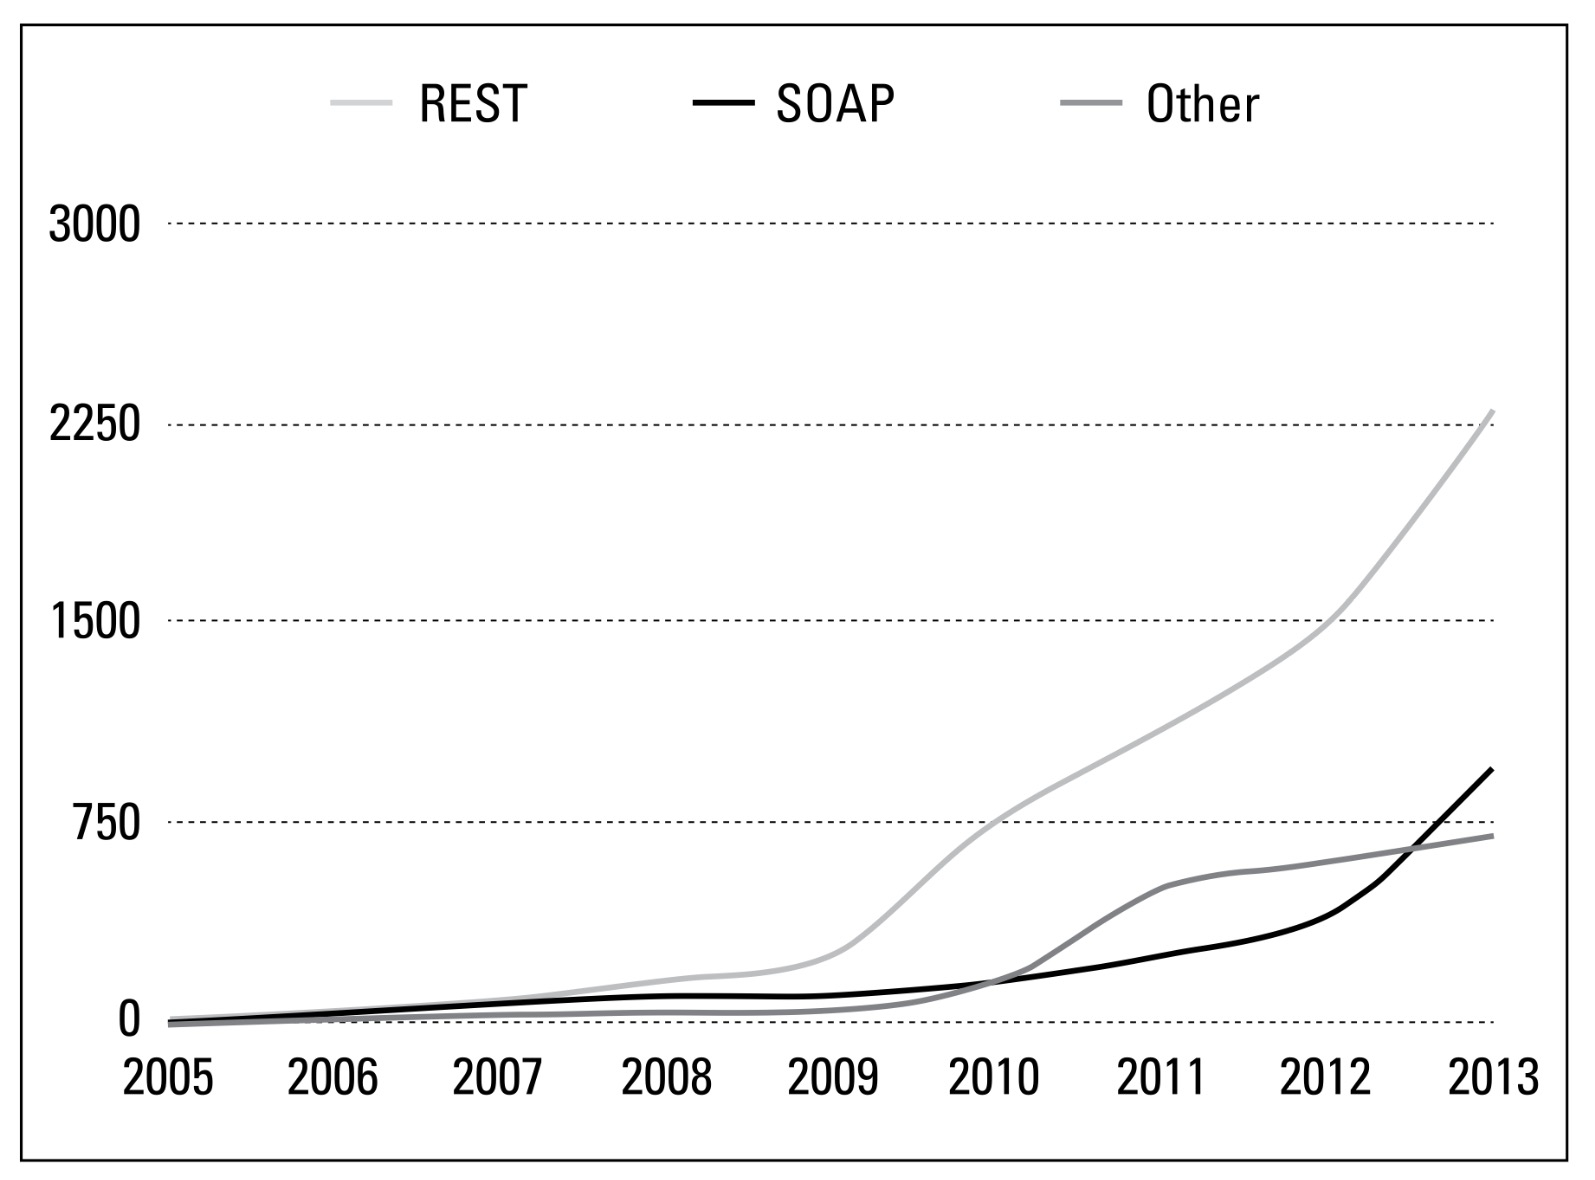
\includegraphics[width=0.9\textwidth,height=\textheight,keepaspectratio]{figuras/api-styles.jpg}
  \caption{Distribuição de estilos e protocolos para APIs}
\end{figure}
% CITAR A FIGURA NO TEXTO

A seguir será apresentada uma visão geral sobre as restrições propostas por Fielding para a implementação em arquiteturas web, além de ser examinado o impacto de cada restrição nesses sistemas distribuídos. \\

\textbf{Cliente-Servidor} \\

Nesta primeira restrição, não existe conexão entre cliente e servidor, mas sim a espera do servidor por pedidos de clientes através de chamada e resposta. O cliente (consumidor do serviço) não se preocupa com tarefas de comunicação de banco de dados, gerenciamento de cache, entre outros. O mesmo ocorre como o servidor (prestador de serviços), que não está preocupado com as tarefas do cliente como interface ou experiência do usuário, por exemplo. Isso permite a evolução independente dos dois ambientes, desde que a interface usada para comunicação entre o cliente e o servidor não seja alterada. \cite{Fielding2000} \\

\textbf{Sem Estado} \\

Esta restrição ajuda na viabilidade, confiabilidade e escalabilidade de sistemas distribuídos, pois garante que chamadas à API não estejam vinculadas a um determinado servidor. Como HTTP é um protocolo sem conexão, cada requisição deve conter todas as informações necessárias para que um servidor entenda o que um cliente está executando. Para Wildermuth, no entanto, dependendo da diversidade no número de clientes, ao manter um servidor sem estado, perder-se o controle no tamanho da estrutura de resposta necessária para atender a demanda de todos os clientes. \cite{Wildermuth2015} \\

\textbf{Interface Uniforme} \\

Em essência, Fielding propõe que aplicações façam o uso de verbos HTTP (POST, GET, PUT, DELETE) e identificadores uniformes de recursos (URIs) para mapear operações em ambientes distribuídos e minimizar o acoplamento entre cliente-servidor. Essas regras de acesso são: \cite{Fielding2000}

\begin{itemize}[noitemsep]
\item Identificação de Recursos: Cada recurso deve ser disponibilizado através de uma URI específica e coesa. (Exemplo: GET /customers/1)
\item Manipulação de Recursos através de Representações: Um recurso pode ser representado em diferentes formatos para diferentes clientes. (Exemplo: HTML, XML, JSON)
\item Resposta Auto-explicativa: Metadados devem ser adicionados na requisição e resposta de um recurso para descrever seu estado atual ou desejado. (Exemplo: código de resposta HTTP, Host, Content-Type)
\item HATEOAS (
 \textit{Hypermedia as the Engine of Application State}): Caso um recurso possua relacionamentos, ao ser representado, estes devem estar especificados em forma de \textit{hyperlinks} para facilitar a navegação de dados por clientes.
\end{itemize}

\textbf{Separação em Camadas} \\

Um dos princípios desta restrição está em evitar que clientes façam diretamente requisição para o servidor sem antes passar por um intermediário, como por exemplo um balanceador de caga (\textit{load balancer})\footnote{
  Técnica para distribuir a carga de trabalho uniformemente entre dois ou mais computadores
}. Desse modo, fica assegurado que clientes apenas se preocupem com a comunicação, deixando que intermediários lidem com a distribuição de requisições. \cite{Fielding2000} \\

\textbf{Código sob Demanda} \\

Apesar de ser a única restrição opcional do estilo, ela permite que servidores disponibilizem código em forma de script para que seja executado no cliente. Dessa forma, a lógica de serviço do servidor é estendida para seus clientes. \cite{Fielding2000} \\

\textbf{Cache} \\

Visa aumentar o desempenho de um serviço. Quando um recurso é acessado por mais de um cliente, se não houve mudança é recomendado que a resposta seja armazenada em cache, evitando o processamento desnecessário. Isso significa que servidores, quando possível, devem implementar regras de cache para beneficio de ambos os ambientes. \cite{Fielding2000}

\section[Descrição de API REST]{Descrição de API REST}

Atualmente, o processo de descrição de APIs tem-se tornado um dos principais fatores de sucesso na aceitação de serviços por desenvolvedores. No entanto, diferente do processo de implementação, a prática de descrição de APIs REST ainda continua sendo feita em sua maior parte manualmente através de linguagem natural. Isso porque REST não apresenta uma forma de documentação externa para descrição de pontos de acesso. \cite{LuckyEtAl2016}

Ao invés, Fielding propõe a descrição dinâmica de APIs através do uso de hiperlinks na representação de recursos para navegação de dados (HATEOAS). Contudo, para Knupp, a solução proposta por Fielding é questionável, pois na sua visão dificulta a legibilidade da interface de acesso, não prevê documentação, cria complexidade de implementação e aumenta de forma significativa o tamanho de resposta. \cite{Knupp2016}

Em busca de oferecer uma solução simples e completa para descrição de APIs REST, foram introduzidas nos últimos anos diversas soluções por empresas e comunidades de desenvolvimento. A seguir, são descritas três das linguagens e formatos que maior ganharam popularidade devido a sua facilidade de uso e legibilidade por humanos e máquinas. \cite{Sandoval2015}

\begin{description}[leftmargin=8em,style=nextline]
  \item[\textbf{OpenAPI}] 
    \begin{enumerate}
        \item[\textbf{+}] Amplamente adotada, ampla comunidade, suporte à diversas linguagens.
        \item[\textbf{$-$}] Carece de especificações avançadas de metadados.
    \end{enumerate}
  \item[\textbf{RAML}] 
    \begin{enumerate}
      \item[\textbf{+}] Suporte à especificação avançada de metadados, adoção significativa, formato legível, suporte da indústria.
       \item[\textbf{$-$}] Falta de ferramentas de auxílio, não comprovada à longo prazo.
    \end{enumerate}
  \item[\textbf{API Blueprint}] 
    \begin{enumerate}
      \item[\textbf{+}] Fácil de entender e simples de escrever.
       \item[\textbf{$-$}] Pouca adoção, carece de especificações avançadas de metadados, difícil de executar.
    \end{enumerate}
\end{description}

Como ainda não existe uma padronização de formato (externo) para descrição de APIs, novas tecnologias estão sujeitas à surgir para melhor se adaptar a comunidade de desenvolvimento. Uma delas, não mencionada anteriormente é o JSON Hyper-Schema que, recentemente através de Lynn e Leach, mostrou ser um método simples e completo para modelagem de APIs REST. Uma vez que possui suporte à descrição de representação de entrada e saída, relacionamentos, HATEOAS, URIs e verbos HTTP  \cite{LynnEtAl2016} \cite{Leach2014}.

